\documentclass[a4paper]{article}

\usepackage{caption}
\usepackage{amsmath}

\captionsetup[table]{position=bottom}

%\usepackage[cm]{fullpage}

% some very useful LaTeX packages include:

%\usepackage{cite}      % Written by Donald Arseneau
                        % V1.6 and later of IEEEtran pre-defines the format
                        % of the cite.sty package \cite{} output to follow
                        % that of IEEE. Loading the cite package will
                        % result in citation numbers being automatically
                        % sorted and properly "ranged". i.e.,
                        % [1], [9], [2], [7], [5], [6]
                        % (without using cite.sty)
                        % will become:
                        % [1], [2], [5]--[7], [9] (using cite.sty)
                        % cite.sty's \cite will automatically add leading
                        % space, if needed. Use cite.sty's noadjust option
                        % (cite.sty V3.8 and later) if you want to turn this
                        % off. cite.sty is already installed on most LaTeX
                        % systems. The latest version can be obtained at:
                        % http://www.ctan.org/tex-archive/macros/latex/contrib/supported/cite/
\usepackage[inline]{enumitem}

\usepackage{graphicx}   % Written by David Carlisle and Sebastian Rahtz
                        % Required if you want graphics, photos, etc.
                        % graphicx.sty is already installed on most LaTeX
                        % systems. The latest version and documentation can
                        % be obtained at:
                        % http://www.ctan.org/tex-archive/macros/latex/required/graphics/
                        % Another good source of documentation is "Using
                        % Imported Graphics in LaTeX2e" by Keith Reckdahl
                        % which can be found as esplatex.ps and epslatex.pdf
                        % at: http://www.ctan.org/tex-archive/info/

%\usepackage{psfrag}    % Written by Craig Barratt, Michael C. Grant,
                        % and David Carlisle
                        % This package allows you to substitute LaTeX
                        % commands for text in imported EPS graphic files.
                        % In this way, LaTeX symbols can be placed into
                        % graphics that have been generated by other
                        % applications. You must use latex->dvips->ps2pdf
                        % workflow (not direct pdf output from pdflatex) if
                        % you wish to use this capability because it works
                        % via some PostScript tricks. Alternatively, the
                        % graphics could be processed as separate files via
                        % psfrag and dvips, then converted to PDF for
                        % inclusion in the main file which uses pdflatex.
                        % Docs are in "The PSfrag System" by Michael C. Grant
                        % and David Carlisle. There is also some information
                        % about using psfrag in "Using Imported Graphics in
                        % LaTeX2e" by Keith Reckdahl which documents the
                        % graphicx package (see above). The psfrag package
                        % and documentation can be obtained at:
                        % http://www.ctan.org/tex-archive/macros/latex/contrib/supported/psfrag/

%\usepackage{subfigure} % Written by Steven Douglas Cochran
                        % This package makes it easy to put subfigures
                        % in your figures. i.e., "figure 1a and 1b"
                        % Docs are in "Using Imported Graphics in LaTeX2e"
                        % by Keith Reckdahl which also documents the graphicx
                        % package (see above). subfigure.sty is already
                        % installed on most LaTeX systems. The latest version
                        % and documentation can be obtained at:
                        % http://www.ctan.org/tex-archive/macros/latex/contrib/supported/subfigure/

\usepackage{url}        % Written by Donald Arseneau
                        % Provides better support for handling and breaking
                        % URLs. url.sty is already installed on most LaTeX
                        % systems. The latest version can be obtained at:
                        % http://www.ctan.org/tex-archive/macros/latex/contrib/other/misc/
                        % Read the url.sty source comments for usage information.

%\usepackage{stfloats}  % Written by Sigitas Tolusis
                        % Gives LaTeX2e the ability to do double column
                        % floats at the bottom of the page as well as the top.
                        % (e.g., "\begin{figure*}[!b]" is not normally
                        % possible in LaTeX2e). This is an invasive package
                        % which rewrites many portions of the LaTeX2e output
                        % routines. It may not work with other packages that
                        % modify the LaTeX2e output routine and/or with other
                        % versions of LaTeX. The latest version and
                        % documentation can be obtained at:
                        % http://www.ctan.org/tex-archive/macros/latex/contrib/supported/sttools/
                        % Documentation is contained in the stfloats.sty
                        % comments as well as in the presfull.pdf file.
                        % Do not use the stfloats baselinefloat ability as
                        % IEEE does not allow \baselineskip to stretch.
                        % Authors submitting work to the IEEE should note
                        % that IEEE rarely uses double column equations and
                        % that authors should try to avoid such use.
                        % Do not be tempted to use the cuted.sty or
                        % midfloat.sty package (by the same author) as IEEE
                        % does not format its papers in such ways.
\usepackage{amssymb}
\usepackage{amsmath}    % From the American Mathematical Society
                        % A popular package that provides many helpful commands
                        % for dealing with mathematics. Note that the AMSmath
                        % package sets \interdisplaylinepenalty to 10000 thus
                        % preventing page breaks from occurring within multiline
                        % equations. Use:
%\interdisplaylinepenalty=2500
                        % after loading amsmath to restore such page breaks
                        % as IEEEtran.cls normally does. amsmath.sty is already
                        % installed on most LaTeX systems. The latest version
                        % and documentation can be obtained at:
                        % http://www.ctan.org/tex-archive/macros/latex/required/amslatex/math/
\usepackage{latexsym}
\usepackage{amsthm}

\usepackage[utf8]{inputenc}
\usepackage[italian]{babel}

\usepackage{algorithm}
\usepackage{algpseudocode}
\algrenewcommand{\algorithmiccomment}[1]{$\left(\text{#1}\right)$}

\usepackage{color}

\definecolor{ideanumber}{rgb}{0.0,0.0,1.0}
\definecolor{ideacomment}{rgb}{0.5,0.5,0.5}
\definecolor{ideakeyword}{rgb}{0.0,0.0,0.5}
\definecolor{ideastring}{rgb}{0.0,0.5,0.0}

\usepackage{listings}
\lstset{frame=tb,
    language=Java,
    aboveskip=3mm,
    belowskip=3mm,
    showstringspaces=false,
    columns=flexible,
    basicstyle={\small\ttfamily},
    numbers=left,
    numbersep=2pt,                   % how far the line-numbers are from the code
    numberstyle=\tiny\color{ideacomment},
    keywordstyle=\color{ideakeyword},
    commentstyle=\color{ideacomment},
    stringstyle=\color{ideastring},
    breaklines=true,
    breakatwhitespace=true,
    tabsize=4
}

% Other popular packages for formatting tables and equations include:

%\usepackage{array}
% Frank Mittelbach's and David Carlisle's array.sty which improves the
% LaTeX2e array and tabular environments to provide better appearances and
% additional user controls. array.sty is already installed on most systems.
% The latest version and documentation can be obtained at:
% http://www.ctan.org/tex-archive/macros/latex/required/tools/

% V1.6 of IEEEtran contains the IEEEeqnarray family of commands that can
% be used to generate multiline equations as well as matrices, tables, etc.

% Also of notable interest:
% Scott Pakin's eqparbox package for creating (automatically sized) equal
% width boxes. Available:
% http://www.ctan.org/tex-archive/macros/latex/contrib/supported/eqparbox/

% *** Do not adjust lengths that control margins, column widths, etc. ***
% *** Do not use packages that alter fonts (such as pslatex).         ***
% There should be no need to do such things with IEEEtran.cls V1.6 and later.
\newcommand\textsup[1]{$^{\text{#1}}$}
\newcommand\textsub[1]{$_{\text{#1}}$}

% Define document title and author
\title{\LARGE \bf
Assigment \#1 - ``The Game of Life''
}
\author{
    Martina Magnani\\
    \texttt{martina.magnani8@studio.unibo.it}
    \and
    Nicola Piscaglia\\
    \texttt{nicola.piscaglia2@studio.unibo.it}
    \and
    Mattia Vandi\\
    \texttt{mattia.vandi@studio.unibo.it}
}
\date{}

% Your document starts here!
\begin{document}

\maketitle

\section{Analisi del problema}\label{analisi-del-problema}

L'obiettivo della consegna è implementare, in Java, una versione concorrente del gioco \textit{``The Game of Life''} usando la programmazione concorrente multi-threaded.\\
Il gioco consiste nel calcolare e visualizzare l'evoluzione della matrice di celle che caratterizza il gioco, come sequenza di fotogrammi (ognuno dei quali rappresenta lo stato del mondo).\\
Nella matrice, ogni cella può essere in uno dei due stati possibili, \textit{live} o \textit{dead}.\\
Dato lo stato \(s\left(t\right)\) della matrice, lo stato \(s\left(t + 1\right)\) si computa con le seguenti regole:

\begin{itemize}
\item
  una cella \(m\left[i,j\right]\) che nello stato \(s\left(t\right)\) è \textit{live} e ha zero o al più una cella vicina \textit{live} (e le altre \textit{dead}), nello stato \(s\left(t + 1\right)\) diventa \textit{dead} (``muore di solitudine'')
\item
  una cella \(m\left[i,j\right]\) che nello stato \(s\left(t\right)\) è \textit{live} e ha quattro o più celle vicine \textit{live}, nello stato \(s\left(t + 1\right)\) diventa \textit{dead} (``muore di sovrappopolamento'')
\item
  una cella \(m\left[i,j\right]\) che nello stato \(s\left(t\right)\) è \textit{live} e ha due o tre celle vicine \textit{live}, nello stato \(s\left(t + 1\right)\) rimane \textit{live} (``sopravvive'')
\item
  una cella \(m\left[i,j\right]\) che nello stato \(s\left(t\right)\) è \textit{dead} e ha tre celle vicine \textit{live}, nello stato \(s\left(t + 1\right)\) diventa \textit{live}
\end{itemize}
Il gioco deve presentare un'interfaccia grafica con pulsanti \texttt{start} e \texttt{stop} con cui si fa partire e fermare il gioco.
Ogni stato del gioco deve essere visualizzato, insieme al numero di celle nello stato \textit{live}.

\subsection{Requisiti del sistema}\label{requisiti-del-sistema}

\begin{itemize}
\item
  Il programma deve funzionare anche con matrici di dimensioni significative (ad es. 5000x5000);
\item
  Massimizzare il throughput, minimizzando il tempo di calcolo di ciascun fotogramma ed eventualmente anche della sequenza di fotogrammi;
\item
  Massimizzare la reattività della GUI;
\item
  Studiare e implementare meccanismi di coordinazione/sincronizzazione basati su semafori o monitor.
\end{itemize}

\section{Descrizione della soluzione proposta}\label{descrizione-della-soluzione-proposta}

\subsection{Architettura del sistema}\label{architettura-del-sistema}

L'architettura del sistema è stata scomposta in tre livelli utilizzando il pattern Model View Presenter con modello ad Interattori, di conseguenza vi sono tre moduli: il dominio applicativo, gli interattori e l'interfaccia grafica:

\begin{itemize}
\item
  Nel primo livello vi è una rappresentazione object-oriented delle componenti del problema;
\item
  Nel secondo livello è stata incapsulata la logica di aggiornamento del gioco;
\item
  Nel terzo livello viene organizzata l'interfaccia grafica che permette la visualizzazione del gioco e l'interazione con l'utente.
\end{itemize}

\subsection{Implementazione}\label{implementazione}

\subsubsection{Dominio applicativo}\label{dominio-applicativo}

Abbiamo implementato il dominio applicativo attraverso due classi:
\texttt{Cell} e \texttt{Board}.\\
L'enumerazione \texttt{Cell} rappresenta lo stato di una cella della scacchiera che può essere \textit{live} o \textit{dead}.
La classe \texttt{Board} rappresenta la scacchiera di gioco. Questa è caratterizzata da un'\textit{altezza} e una \textit{larghezza} variabili e dalla possibilità di recuperare/impostare lo stato di una cella date le coordinate $x$ e $y$.

\subsubsection{Interattori}\label{interattori}

Abbiamo implementato un interattore \texttt{BoardUpdater} che si occupa dell'aggiornamento della scacchiera di gioco. Di questo interattore ne esistono due versioni, una sequenziale e una concorrente.

La versione sequenziale (\texttt{SequentialBoardUpdater}) l'aggiornamento della schermata di gioco viene eseguito sul thread corrente senza la creazione di nuovi thread.

Nella versione concorrente \texttt{ConcurrentBoardUpdater} è possibile configurare il numero di \texttt{Worker} che verranno utilizzati per aggiornare la schermata di gioco (ognuno dei quali verrà eseguito su un thread indipendente).\\
Il metodo \texttt{start} si occupa della creazione di un nuovo thread per ogni \texttt{Worker} e di metterlo in esecuzione.\\
Il metodo \texttt{stop} si occupa di terminare l'esecuzione dei \texttt{Worker}.\\
Il metodo \texttt{update} gestisce l'aggiornamento della scacchiera di gioco (board). Per prima cosa si occupa di creare una nuova scacchiera che rappresenterà lo stato della scacchiera corrente dopo l'aggiornamento. Successivamente divide il lavoro fra i \texttt{Worker} cercando di bilanciarlo il più possibile. Dopodiché sospende la propria esecuzione in attesa che tutti i \texttt{Worker} abbiano terminato l'aggiornamento della porzione di scacchiera assegnatagli.\\
Ogni \texttt{Worker}, appena messo in esecuzione, aspetta che gli venga assegnata la porzione di scacchiera da aggiornare. Una volta terminata l'attesa, se ancora in esecuzione, effettua l'aggiornamento delle celle seguendo le regole del gioco (indicate nell'analisi del problema). Una volta terminato il lavoro, il \texttt{Worker} lo segnala al \texttt{CuncurrentBoardUpdater} di aver terminato l'aggiornamento della propria porzione di scacchiera e si mette in attesa di essere eseguito nuovamente.

Per ogni \texttt{Worker} la sincronizzazione con \texttt{CuncurrentBoardUpdater} è effettuata tramite due semafori binari: il primo (\texttt{startUpdate}) viene utilizzato per segnalare al \texttt{Worker} che può iniziare l'aggiornamento della propria porzione di scacchiera, il secondo (\texttt{finishedUpdate}) viene utilizzato per segnalare al \texttt{CuncurrentBoardUpdater} che il \texttt{Worker} ha terminato l'aggiornamento della sua porzione di scacchiera.

In questo modo \texttt{ConcurrentBoardUpdateer} segnala ad ogni \texttt{Worker} che la relativa porzione di scacchiera è pronta per essere aggiornata. Così attende che ogni \texttt{Worker} finisca il proprio lavoro per poi restituire la nuova scacchiera.

\subsubsection{Interfaccia utente}\label{interfaccia-utente}

L’interfaccia utente è stata realizzata con Java FX ed è costituita da due schermate: nella prima si permette all’utente di settare le dimensioni della scacchiera di gioco (altezza e larghezza) ed il numero di \texttt{Worker}. Nella seconda si visualizza la scacchiera e sono presenti due pulsanti \textit{start} e \textit{stop}. Lo \textit{start} permette l’avvio e la pausa del gioco, mentre lo \textit{stop} la terminazione.\\
Utilizzando il pattern Factory sono stati incapsulate in una apposita classe le funzioni per la costruzione delle finestre grafiche. Le callback di queste finestre sono definite da opportuni \texttt{Presenter} che incapsulano la logica di controllo dei componenti (form, pulsanti, …) di cui sono costituite.\\
La computazione relativa alla coordinazione dell’aggiornamento matriciale e grafico della scacchiera è effettuata su un thread separato \texttt{GameUpdater} (task di Java FX in cui è incapsulato il Game Loop) e questo permette di mantenere l’interfaccia grafica (gestita dal Java FX Application Thread) reattiva ed in grado di intercettare l’input dell’utente.\\
Il Presenter addetto alla gestione degli eventi di gioco (\texttt{GamePresenter}) utilizza un servizio di rendering offerto dalla  classe \texttt{RenderingService} nella quale sono state incapsulate le funzioni relative al disegno della scacchiera di gioco.
Quest'ultima è stata realizzata utilizzando un componente grafico \texttt{Canvas} sul quale vengono disegnate le celle attraverso la classe \texttt{PixelWriter} di Java FX: una classe ottimizzata per il disegno dei singoli pixel.

\section{Dinamica del sistema}\label{dinamica-del-sistema}
La dinamica del sistema è stata rappresentata formalmente con le Reti di Petri. Le piazze (\textit{places}) del livello corrispondono ai \texttt{Worker} che concorrono all'aggiornamento della scacchiera di gioco; in questo esempio è stato scelto di mostrare il sistema nel caso se ne utilizzino 4.
\begin{figure}[H]
    \centering
    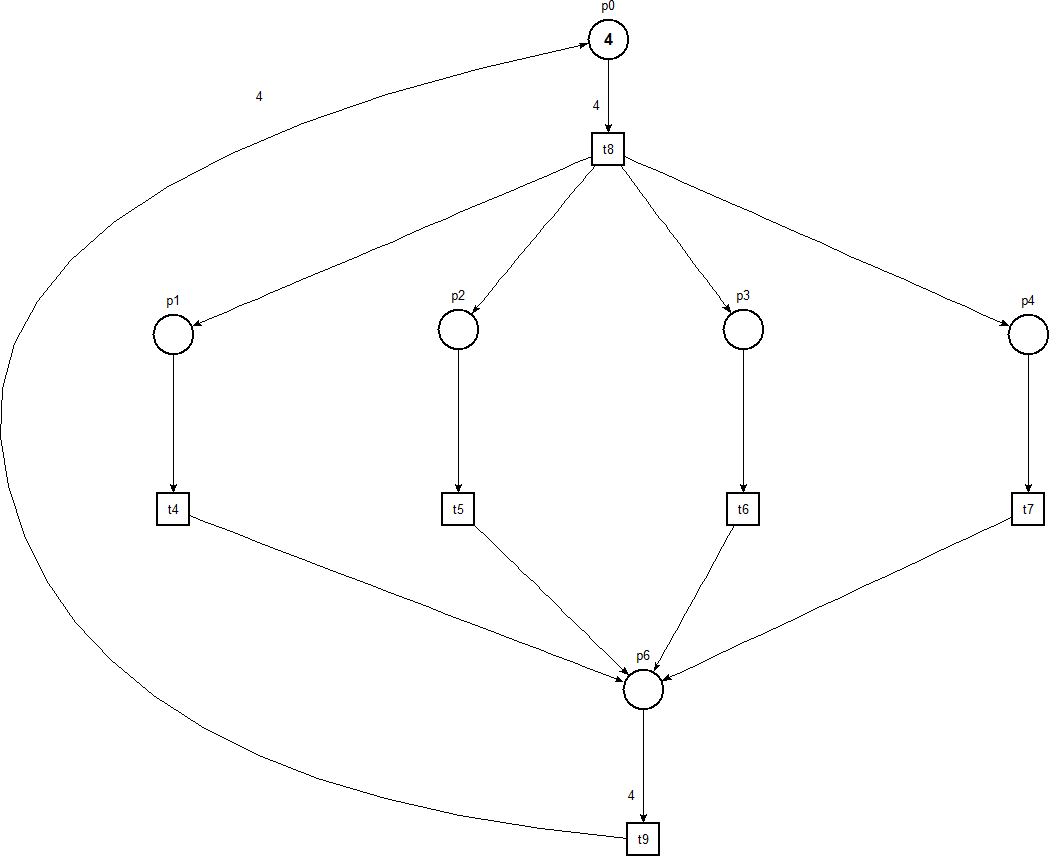
\includegraphics[width=110mm]{res/reti_di_petri_assigment1.png}
    \caption{Petri Net}
    \label{fig:petrinets}
\end{figure}

\section{Analisi delle prestazioni}\label{analisi-delle-prestazioni}
La tabella sottostante mostra gli speedup $S$ (misura quantitativa delle performance) che il sistema raggiunge a seconda del numero di worker utilizzati.\\
Lo speedup viene misurato calcolando il rapporto tra il tempo di esecuzione del sistema utilizzando un algoritmo sequenziale e il tempo di esecuzione del sistema utilizzando un algoritmo parallelo.

\begin{equation}
 S = \frac{T_1}{T_N}
\end{equation}
Dove:
\begin{itemize}
    \item $N \leftarrow$ numero di worker utilizzati
    \item $T_1 \leftarrow$ tempo di esecuzione del sistema utilizzando un algoritmo sequenziale
    \item $T_N \leftarrow$ tempo di esecuzione del sistema utilizzando un algoritmo parallelo con $N$ worker
\end{itemize}

\begin{table}[H]
\centering
\begin{tabular}{l|ccccccccc}
\hline
     & 2     & 3    & 4    & 5    & 6    & 7    & 8    & 9    & 10   \\ \hline
Min. & 1.77  & 2.43 & 3.04 & 2.93 & 2.89 & 2.90 & 2.86 & 2.85 & 2.85 \\
Max. & 2.11  & 2.87 & 3.41 & 3.22 & 3.40 & 3.26 & 3.38 & 3.06 & 3.45 \\
Avg. & 1.81  & 2.50 & 3.06 & 2.94 & 2.93 & 2.91 & 2.92 & 2.85 & 2.94 \\ \hline
\end{tabular}
\caption{Speedup considerando schacchiera di gioco 5000x5000: sulle colonne sono specificati il numero di worker utilizzati per la parallelizzazione dell'algoritmo, sulle righe i valori statistici (minimi, massimi e medi) degli speedup calcolati. Gli speed-up sono stati calcolati su un Apple Macbook Pro (Retina, 15", metà 2015) dotato di un processore Intel Core i7 quad-core a 2.2GHz.}
\label{Tabella speedup del sistema}
\end{table}

% Your document ends here!
\end{document}
